\section{Future Work}
\label{sec:conclusions:future}

\subsection{For Other Factorization}
\label{ssec:future:other-factorization}
In this thesis, we mainly focus on the independent factorization,
which ignores the interdependence between output parts.  Our
experiments shows contexturalized representation capturing the
interdependence within the input parts can still offer discriminative
features to independently predict each local output parts. However,
there are other factorizations we can extend our work on, such as
auto-regressive factorization, or arbitrary high order
factorizations. In those cases, the output parts will either depend on
the previously predicted output, or have other high order
dependecies. Take the auto-regressive factorization as an example, we
consider a more broad-coverage construction of output \OUT~as
sequential decisions as shown in~\autoref{eq:auto-factor}.

\begin{equation}
  \label{eq:auto-factor}
E(x, y)=\sum_{j=0}^{M}E(y_{j}|x,y_{<j})
\end{equation}

In autoregressive factorization, as shown in
~\autoref{fig:autoreg-example}, for every step, a new decision $y_{j}$
will depend on the input $x$ and previous decisions $y_{<j}$. In this
case, the main challenge of the model is to learn the representation
of $x$ and previous sequential decisions $y_{<j}$, then make a
decision $y_{j}$ based on them.  Especially inspired by distributed
representation of the natural language, we also study the distributed
representation of the output structures $y_{<j}$, and leverage them to
guide constrained structured prediction.

\begin{figure}[h]
\centering
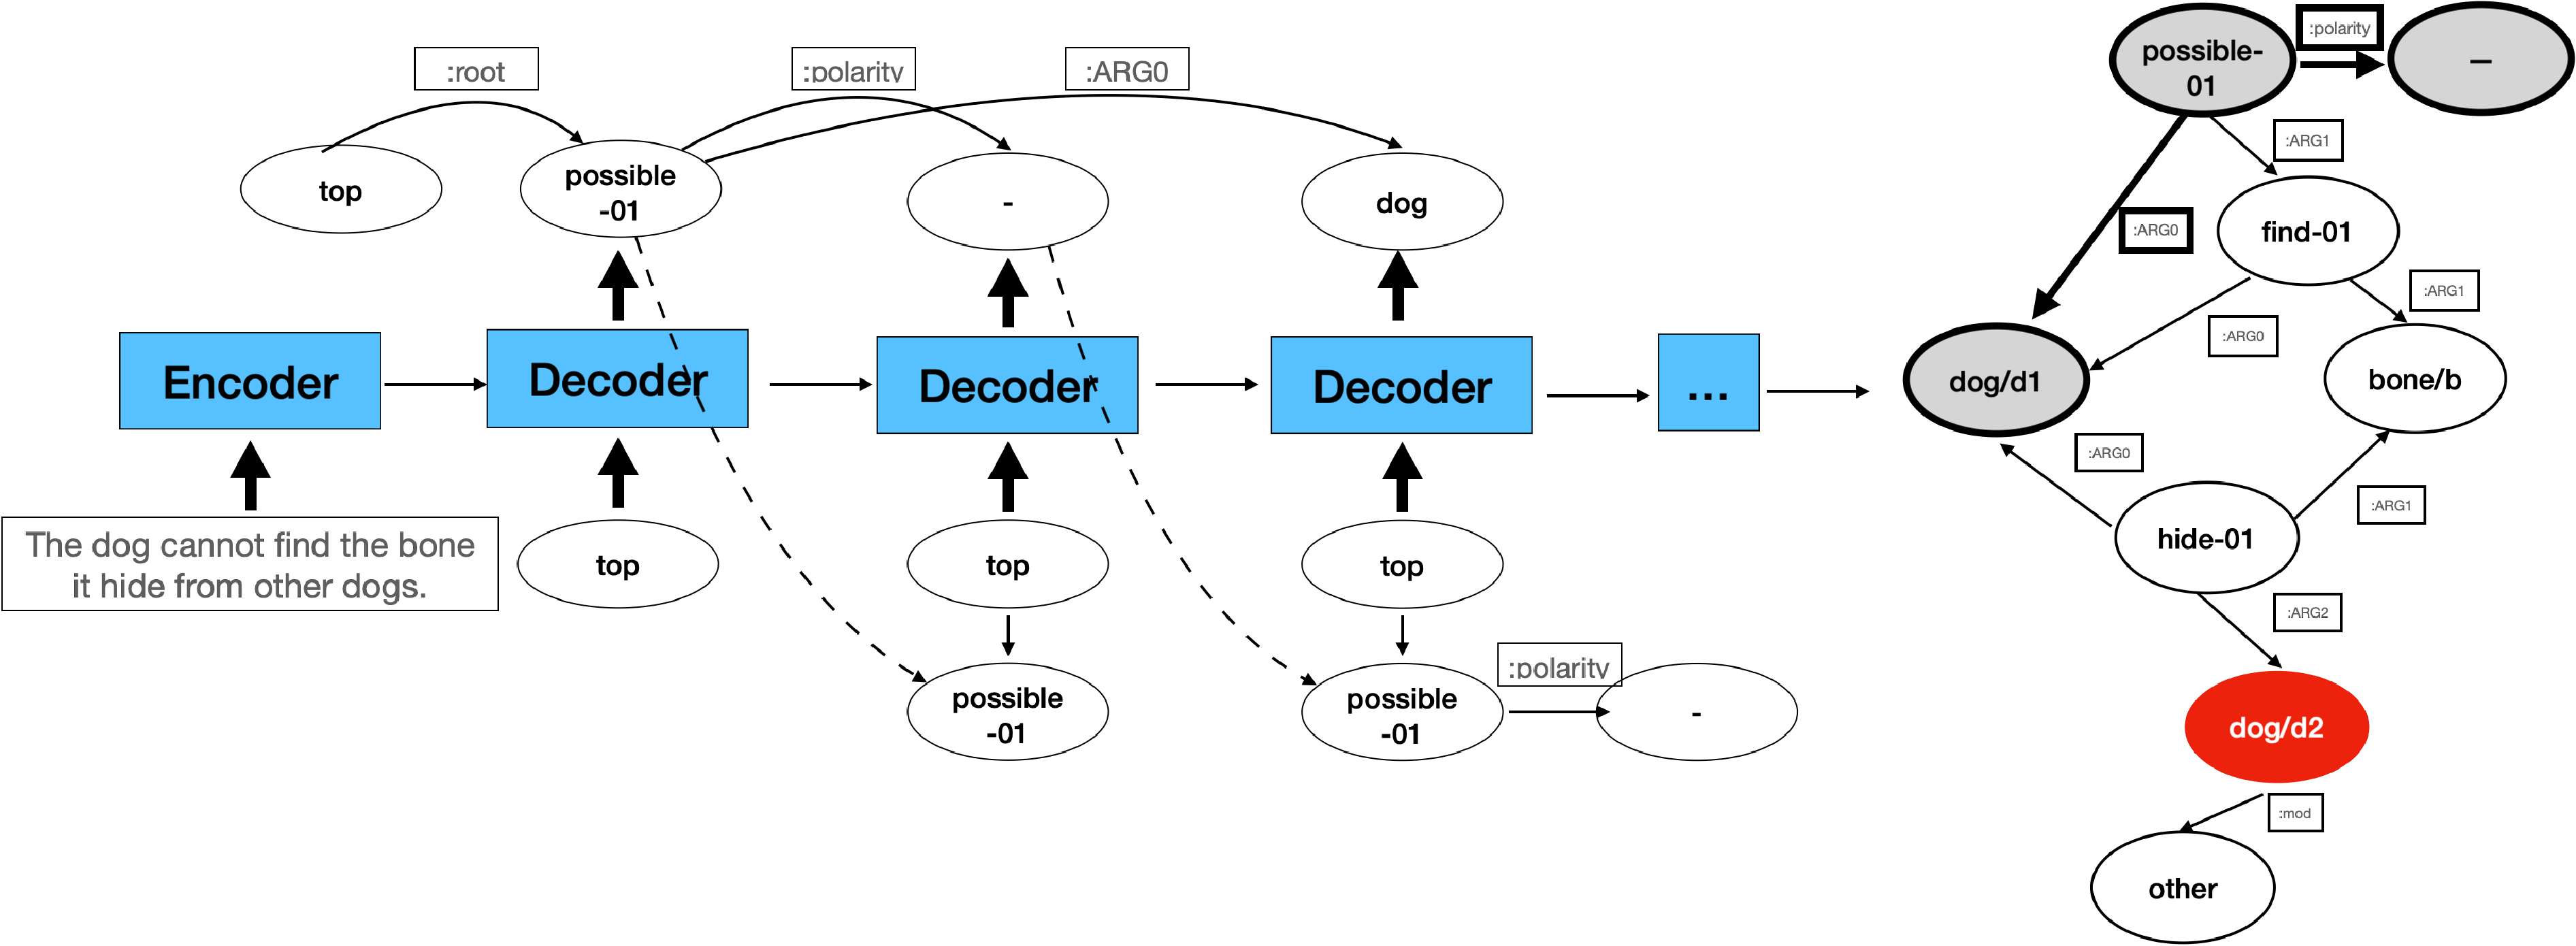
\includegraphics[width=0.92\textwidth]{seq2graph.pdf}
\caption{\label{fig:autoreg-example}The autoregressive factorization
  of AMR Parsing in different decoding time step}
\end{figure}

\subsection{Apply to Other Symbolic Representations}
\label{ssec:future:application}
As shown in~\autoref{chap:leixcal-phrasal}, above structural inductive
bias in lexical, phrasal, sentential anchoring can be easily extended
to other linguistic structured prediction tasks, such as coreference
resolution, semantic role labeling, where the main task strutures has
been studied in our broad-coverage meaning representation parsing.

For application-specific symbolic representation, besides the single
sentence representation
in~\cite[TOP,][]{gupta-etal-2018-semantic-parsing}, we also can extend
our structured prediction models into session-based conversational
representation such as session-based
TOP~\cite{aghajanyan2020conversational},
~\cite[TreeDST,][]{cheng2020conversational}, and
~\cite[Dataflow,][]{andreas2020task}.  Beyond conversational analysis,
in the future, I plan to exploit this structured analysis on symbolic
representation to offer rigorous document analysis, easier knowledge
organization, programmable reasoning, which are potentially helpful
for structured social analysis such as mental health, cyberbullying,
thus offering structural suggestions to guide human behavior.

\subsection{Future Work on Contexualized Representation}
\label{ssec:future:contextural-rep} The strong power of
contexturalized representation learning make out independent
factorization works still gold under our inductive biases. However,
there are still many challenges on contexturalized representation
learning.

\Paragraph{Extreme Long Context} First, we need to resolve extrem long
text encoding problem. Our current models on psychotherapy dialogue
and schema-guided dialog only consider 8 to 16 utterance as the
dialogue history window. However, we have more than 500 utterance in a
single therapy session. Further more, a psychotherapy treatment may
last for months and years, which involves multiple dialogue
sessions. The long context problem also exists in other domain, such
as scientific document analysis, and threaded conversations in social
medias.

\Paragraph{Contextualized Representation Beyond Text} multimodality

\subsection{Other Biases in Other Formalism}
\label{ssec:future:rep-bias-ways}

Besides the above structural inductive bias on compositionality and
hierarchial structure, in the future, I will continue the study on how
to represent other inductive biases in other ways.

\Paragraph{Declaritive Constraints and other latent Models}In the
future, we also inject other structural interdependence/constraints
with declaritive tools, such as integer linear programming,
probabilistic neural logic rules. Further more, following the line of
latent variable models, we plan to study more ways to relax structural
inductive biases as continuous and differentiable latent variables in
the end2end deep learning.

\Paragraph{Approximate Bias} With limited observations and
resources~(time, memory, energy), our human intelligence of
generalizing to new environments makes us efficiently learn when
interacting with the world and other human beings. This efficiency
largely depends on many \kw{inductive biases} and \kw{approximate
  biases} from human intelligence~\cite{Gershman2021WhatMU}, which are
potentially helpful for machine intelligence. We also plan to working
approximate biases for reasoning. Especially, for deep learning, we
plan to design approximate inference methods for deep structured
prediction.

\Paragraph{Causality} Current factorization and markov random field
based formalism only can capture the correlation between different
variables. In the future, we will also extend the formalism to
bayesian networks and intervention based models.

\subsection{Learning and Transfering the Inductive Biases}
\label{ssec:future:bias-learn-transfer}

\Paragraph{Learn the Inductive Biases via Self-supervision}
Inspired by self-supervised pretraining in ELMo and
BERT~\cite{devlin2019bert}, our VLDB'2022
paper~\cite{paul2021database} extend a contrastive-learning method to
learn the representation for tree-structured database query
plans. With a large amount of raw database query plans, we calculate
the graph similarity metric~{\em Smatch}~\cite{Cai:2013wn} to
represent the degree of overlap between a pair of plans.\footnote{The
  Smatch score~([0,1]) between two tree-structure plans can be
  computed by graph matching optimization algorithm, such as Integer
  Linear Programming~(ILP) or Hill-climbing methods.}  After we get
the {\em Smatch} scores $s_{ij}$ of each plan-pair $<p_{i}, p_{j}>$,
this can easily form a large dataset with {\em Smatch} score as the
contrastive self-supervision. In our experiments on the downstream
applications, we show that the structure encoder pre-trained from this
task can be easily finetuned for a new task or domain.

\Paragraph{Transfering Inductive Bias via Supplementary Training}
Learning to learn is an essential inductive bias in human
intelligence~\cite{harlow1949formation}, human can generalize
experience learned from similar tasks to learn new tasks. Nowadays
many datasets and pre-trained models are publicly accessible, besides
transferring the inductive bias from initial language models, I also
studied how to transfer the inductive biases learned from the
well-studied tasks to new tasks. My NAACL'2021 work on schema-guided
dialogue state tracking~\cite{cao2021schema} proposed to add a
supplementary pretraining phase on an intermediate task between the
pretraining-finetuning framework. Given a brand new task like
schema-guided dialogue state tracking, we show that supplementary
pretraining on intermediate tasks with similar problem structures will
offer efficient distributional inductive biases. More specifically, we
found that inductive bias learned in sentence-pair matching~(via
Natural Language Inference on SNLI) helps with intent classification
tasks, and span-based retrieval task structure~(via Question Answering
on SQuAD2) helps on the non-categorical slot labeling task.

Besides passively receiving fixed training data to learn, intelligent
systems can improve themselves by actively discovering more
supervisions. My future work will ground the explorations on two sub
areas:
\begin{inparaenum}[(a)]
\item learning on how to retrieve and integrate the experience with
  new observations. This is similar to how humans learn from the
  experience and other existing tools, including searching over
  similar datasets or pre-trained models.
\item learning on make the model self-evolve, such as via the
  feedback after deployment.
\end{inparaenum}


%%% Local Variables:
%%% mode: latex
%%% TeX-master: "../../thesis-main.ltx"
%%% End:
